\scanpage{129}
\deleted{Or les données 1°, 2° correspondent resp. à des \deleted{sections}\inserted{\unsure{points}} de préschémas affines $\unsure{K_T},\unsure{L_T}$ sur $S$, \inserted{[puisque $Z',X''$ \inserted{propres et} plats sur $S$]} donc 1° et 2° à une section de $K\times L$ sur $S$. \deleted{\unsure{et}} D'autre part, les isom de $(L_1''')_T$ sur $(L_3''')_T$ correspondent aux \deleted{des} sections \deleted{de $R$} un $M_T$ affine, \deleted{sur $S$} et ceux de $\mathcal O_{Z''_T}$ sur $i''_T{}^*(L_1'')$ aux sections d'un $N_T$ affine \deleted{\unsure{sur}} \inserted{[car $X''',Z''$ propres et plats sur $S$]} Les conditions a) et b) s'expriment donc en \deleted{disant} faisant coïncider des morphismes donnés
\diagram{\begin{tikzcd}[column sep=small]
K\arrow[r,shift left=0.6ex]\arrow[r,shift right=0.6ex]&M,&L\arrow[r,shift left=0.6ex]\arrow[r,shift right=0.6ex]&N
\end{tikzcd}}
de $K\times M\rightrightarrows L\times N$. Donc on trouve un sous-présch. fermé de $K\times M$. Cela achève la démonstration.}

\margin{\figure{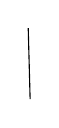
\begin{tikzpicture}[x=0.3cm,y=0.3cm]\draw (0,3)--(0.08,0);\fill (0.055,1.45) circle (0.025);\fill (0.07,0.65) circle (0.025);\end{tikzpicture}}}
\uline{Corollaire}. $X$ séparable et complet sur le corps $k$. \deleted{Supposons les $\underline{\operatorname{Pic}}_{X_i/k}$ existent.}\inserted{\unsure{A}} \deleted{Alors $\underline{\operatorname{Pic}}_{X/k}$ existe.} Soit $X_i$ les composantes \inserted{(réduites)} \deleted{\unsure{des} $X_i$ \unsure{sont irrédu} de $X$}, \deleted{\unsure{sont}} considérons $\underline{\operatorname{Pic}}_{X/k}\text{---}\prod_i\underline{\operatorname{Pic}}_{X_i/k}$, \inserted{cet hom} \deleted{\unsure{trouve} le noyau est affine} \deleted{est affine}. représentable par des morphismes affines. donc si les $\underline{\operatorname{Pic}}_{X_i/k}$ existent, de même $\underline{\operatorname{Pic}}_{X/k}$.
\margin{128}
